\setcounter{deso}{2}
\begin{name}
	{ÔN TẬP KIỂM TRA CUỐI HỌC KÌ 1}
	{TOÁN 10}
	{LỚP TOÁN THẦY PHÁT}
	{\thoigian}
\end{name}
%================================PHẦN I
\caulc
\Opensolutionfile{ans}[ans/0-HK1-CD-2-SoBacGiang-2324-Phan-I]
\begin{ex}%[0H5N2-2]%[VN-MT6, Đào Trung Kiên]%[Sở Bắc Giang]
	Cho bốn điểm bất kì $A$, $B$, $C$, $O$. Đẳng thức nào sau đây đúng?
	\choice
	{$\overrightarrow{AB}=\overrightarrow{AC}+\overrightarrow{BC}$}
	{$\overrightarrow{OA}=\overrightarrow{OB}+\overrightarrow{AB}$}
	{\True $\overrightarrow{OA}=\overrightarrow{CA}+\overrightarrow{OC}$}
	{$\overrightarrow{AB}=\overrightarrow{OB}+\overrightarrow{OA}$}
	\loigiai
	{
		Ta có $\overrightarrow{OA}=\overrightarrow{OC}+\overrightarrow{CA}=\overrightarrow{CA}+\overrightarrow{OC}$.
	}
\end{ex}

\begin{ex}%[BG - 10 New - 3in1, Nguyễn Văn Cường (Cường NV)]%[0D8H1-2]
Có $10$ cặp vợ chồng đi dự tiệc. Tổng số cách chọn một người đàn ông và một người đàn bà trong bữa tiệc phát biểu ý kiến sao cho hai người đó không là vợ chồng?
\choice
{$100$}
{$91$}
{$10$}
{\True $90$}
\loigiai{
Để chọn một người đàn ông và một người đàn bà không là vợ chồng, ta có
\begin{itemize}
\item Có $10$ cách chọn người đàn ông.
\item Có $9$ cách chọn người đàn bà.
\end{itemize}
Vậy theo qui tắc nhân ta có $9 \times 10=90$ cách.
}
\end{ex}

\begin{ex}%[1D1N2-2]%[[0H4N1-2]%[VN-MT6, Đào Trung Kiên]%[Sở Bắc Giang]
	Trong các đẳng thức sau đây, đẳng thức nào đúng?
	\choice
	{$\cot 150^\circ=\sqrt 3$}
	{\True $\cos 150^\circ=-\dfrac{\sqrt 3}{2}$}
	{$\sin 150^\circ=-\dfrac{\sqrt 3}{2}$}
	{$\tan 150^\circ=\dfrac{\sqrt 3}{3}$}
	\loigiai
	{
		Ta có $\cos 150^\circ=-\dfrac{\sqrt 3}{2}$.
	}
\end{ex}

\begin{ex}%[0D1N1-3]%[VN-MT6, Đào Trung Kiên]%[Sở Bắc Giang]
	Mệnh đề phủ định của mệnh đề \lq\lq $\forall x\in\mathbb{R}$, $x^2-4x+5>0$\rq\rq\ là
	\choice
	{\lq\lq $\exists x\in\mathbb{R}$, $x^2-4x+5>0$\rq\rq}
	{\lq\lq $\forall x\in\mathbb{R}$, $x^2-4x+5\leq 0$\rq\rq}
	{\lq\lq $\exists x\in\mathbb{R}$, $x^2-4x+5<0$\rq\rq}
	{\True \lq\lq $\exists x\in\mathbb{R}$, $x^2-4x+5\leq 0$\rq\rq}
	\loigiai
	{
		Mệnh đề phủ định của mệnh đề \lq\lq $\forall x\in\mathbb{R}$, $x^2-4x+5>0$\rq\rq\ là \lq\lq $\exists x\in\mathbb{R}$, $x^2-4x+5\leq 0$\rq\rq.
	}
\end{ex}

\begin{ex}%[0D8N2-1]%[Dự án đề kiểm tra Toán khối 11 HKII NH23-24-Dot15-PhucChuong]%[THPT Nhu Van Lang - Hai Phong]
Công thức tính số chỉnh hợp chập $k$ của $n$ phần tử là:
\choice
{$A_n^k=\dfrac{n!}{\left(n-k\right)!k!}$}
{$C_n^k=\dfrac{n!}{\left(n-k\right)!}$}
{$C_n^k=\dfrac{n!}{\left(n-k\right)!k!}$}
{\True $A_n^k=\dfrac{n!}{\left(n-k\right)!}$}
\loigiai{
Công thức tính số chỉnh hợp chập $k$ của $n$ phần tử là $A_n^k=\dfrac{n!}{\left(n-k\right)!}$.
}
\end{ex}
\begin{ex}%[0H4N2-1]%[VN-MT6, Đào Trung Kiên]%[Sở Bắc Giang]
	Cho tam giác $ABC$ có $AC=b$. Bán kính $R$ của đường tròn ngoại tiếp tam giác $ABC$ được tính bởi công thức nào sau đây?
	\choice
	{$R=\dfrac{2b}{\sin B}$}
	{\True $R=\dfrac{b}{2\sin B}$}
	{$R=\dfrac{\sin B}{b}$}
	{$R=\dfrac{\sin B}{2b}$}
	\loigiai
	{
		Ta có $\dfrac{b}{\sin B}=2R \Leftrightarrow R=\dfrac{b}{2\sin B}$.
	}
\end{ex}

\begin{ex}%[0D2N2-2]%[VN-MT6, Đào Trung Kiên]%[Sở Bắc Giang]
	\immini[thm]
	{Bất phương trình nào sau đây có miền nghiệm là phần \textbf{không} tô đậm (không kể đường thẳng $d$) như hình vẽ?
		\choice[2]
		{$3x-2y>-6$}
		{$3x-2y\geq -6$}
		{\True $3x-2y<-6$}
		{$3x-2y\leq -6$}
	}
	{\begin{tikzpicture}[scale=0.75, font=\footnotesize, line join=round, line cap=round, >=stealth]
			\draw[thick, ->](-3.5,0)--(1,0)node[below]{$x$};
			\draw[thick, ->](0,-1.5)--(0,4)node[left]{$y$};
			\fill[pattern=north west lines, pattern color = blue!70!white] (-3,-1.5)--(1,-1.5)--(1,4)--(2/3,4);
			\draw[smooth, samples=100, domain=-3:2/3]plot(\x,{3/2*(\x)+3});
			\fill[white]
			(-0.35,-0.35)circle(6.5pt)
			;
			\path
			(-0.35,-0.35)node[]{$O$}
			(-2.2,0)node[above]{$-2$}
			(0,3)node[left]{$3$}
			(-1,2)node[]{$d$}
			;
		\end{tikzpicture}
	}
	\loigiai
	{Ta thấy điểm $O(0;0)$ thuộc miền nghiệm của các bất phương trình $3x-2y>-6$ và $3x-2y\geq -6$. \\
		Do đó phần nửa mặt phẳng bờ $d$, không chứa điểm $O$ và không kể đường thẳng $d$ là miền nghiệm của bất phương trình $3x-2y< -6$.}
\end{ex}

\begin{ex}%[0H9N1-4]%[Dự án đề kiểm tra Toán khối 10 HKI NH23-24-Dot 15- Hồ Văn Trung]%[THPT Lê Qúy Đôn- TPHCM]
Trong mặt phẳng $Oxy$, cho $\overrightarrow{a}=\left(-5;0\right)$, $\overrightarrow{b}=\left(4;x\right)$. Tìm giá trị $x$ để hai vectơ $\overrightarrow{a}$ và $\overrightarrow{b}$ cùng phương.
\choice
{$x=-1$}
{\True $x=0$}
{$x=4$}
{$x=-5$}
\loigiai{Để hai vectơ $\vec{a}$, $\vec{b}$ cùng phương thì $-5 \cdot x = 0 \cdot 4 \Rightarrow x=0.$
}
\end{ex}

\begin{ex}%[0H4N2-1]%[VN-MT6, Đào Trung Kiên]%[Sở Bắc Giang]
	Cho tam giác $ABC$ có $AB=2$, $AC=3$ và $\widehat{BAC}=60^\circ$. Độ dài cạnh $BC$ là
	\choice
	{\True $\sqrt{7}$}
	{$\sqrt{19}$}
	{$7$}
	{$\sqrt{13}$}
	\loigiai
	{
		Ta có $BC=\sqrt{AB^2+AC^2-2\cdot AB\cdot AC\cdot\cos\widehat{BAC}}=\sqrt{2^2+3^2-2\cdot2\cdot3\cdot\dfrac{1}{2}}=\sqrt{7}$.
	}
\end{ex}

\begin{ex}%[0H5H4-1]%[VN-MT6, Đào Trung Kiên]%[Sở Bắc Giang]
	Cho tam giác đều $ABC$ có cạnh bằng $a$. Khẳng định nào sau đây đúng?
	\choice
	{$\overrightarrow{AB}\cdot\overrightarrow{BC}=-\dfrac{a^2\sqrt 3}{2}$}
	{$\overrightarrow{AB}\cdot\overrightarrow{BC}=\dfrac{a^2\sqrt 3}{2}$}
	{$\overrightarrow{AB}\cdot\overrightarrow{BC}=\dfrac{a^2}{2}$}
	{\True $\overrightarrow{AB}\cdot\overrightarrow{BC}=-\dfrac{a^2}{2}$}
	\loigiai
	{
		\begin{center}
			\begin{tikzpicture}[font=\footnotesize,line join=round, line cap=round, >=stealth,scale=1]
				\path
				(0,0) coordinate (B)
				(B)+(60:3) coordinate (A)
				(B)+(0:3) coordinate (C)
				;
				\draw (A)--(B)--(C)--cycle ;
				\foreach \x/\g in {A/90,B/180,C/0}\fill[draw,fill=black] (\x) circle (1pt)+(\g:3mm) node{$\x$};
			\end{tikzpicture}
			
		\end{center}
		Ta có $\overrightarrow{AB}\cdot\overrightarrow{BC}=-\overrightarrow{BA}\cdot\overrightarrow{BC}=-\left|\overrightarrow{BA}\right|\cdot\left|\overrightarrow{BC}\right|\cdot\cos\widehat{ABC}=-a\cdot a\cdot\cos 60^\circ=-\dfrac{a^2}{2}$.
	}
\end{ex}

\begin{ex}%[BG - 10 New - 4in1,Phú Thạch]%[0D8N3-4]
Tìm hệ số của số hạng chứa $x^5$ trong khai triển nhị thức $\left(x^2-2x\right)^{4}$.
\choice
{$24$}
{$32$}
{\True$-32$}
{$-8$}
\loigiai{Ta có
\allowdisplaybreaks
\begin{eqnarray*}
(x^2-2x)^4&=&(x^2)^4-4(x^2)^3\cdot 2x+6(x^2)^2\cdot (2x)^2-4x^2\cdot (2x)^3+(2x)^4\\
&=&x^8-8x^7+24x^6-32x^5+16x^4.
\end{eqnarray*}
Do đó hệ số của số hạng chứa $x^5$ là $-32$.
}
\end{ex}

\begin{ex}%[0H9N2-1]
%Câu 9 :
Trong mặt phẳng tọa độ $Oxy$ cho ba điểm $A\left( 3;-1 \right),B\left( 2;10 \right),C\left( -4;2 \right)$. Tính tích vô hướng $\overrightarrow{AB}\cdot \overrightarrow{AC}$.
\choice
{\True $40$}
{$-40$}
{$26$}
{$-26$}
\loigiai{
Ta có \begin{eqnarray*}
\overrightarrow{AB}=\left( -1;11 \right);\;\overrightarrow{AC}=\left( -7;3 \right)
\Rightarrow \overrightarrow{AB}\cdot \overrightarrow{AC}=-1\cdot (-7)+11\cdot 3=40.
\end{eqnarray*}
}
\end{ex}

\Closesolutionfile{ans}
%================================PHẦN II
\cauds
\Opensolutionfile{ans}[ans/0-HK1-CD-2-SoBacGiang-2324-Phan-II]
% \setcounter{ex}{0}

\begin{ex}%[0D8V2-7]
Xếp ngẫu nhiên $5$ bạn gồm $3$ bạn nam và $2$ bạn nữ (trong đó có $1$ bạn nữ tên An và $1$ bạn nam tên Bình) ngồi vào một dãy $5$ ghế thẳng hàng (mỗi bạn ngồi 1 ghế). Các mệnh đề sau đúng hay sai?
\choiceTF
{Có $5!$ cách xếp sao cho An luôn ngồi ở vị trí chính giữa}
{Có $12$ cách xếp sao cho các bạn nam luôn ngồi cạnh nhau và các bạn nữ luôn ngồi cạnh nhau}
{\True Có $48$ cách xếp sao cho An và Bình luôn ngồi cạnh nhau}
{\True Có $3! \cdot 2!$ cách xếp sao cho các bạn nam và nữ luôn ngồi xen kẽ nhau}
\loigiai{
\begin{itemchoice}
\itemch Sai.\\
An luôn ngồi ở vị trí chính giữa: có 1 cách xếp.\\
Xếp 4 bạn còn lại vào 4 vị trí còn lại: có $4!$ cách xếp.\\
Vậy có $4!$ cách xếp sao cho An luôn ngồi ở vị trí chính giữa.
\itemch Sai.\\
Có 2 cách xếp vị trí cho nam và nữ.\\
Trong mỗi cách trên, có $3!$ cách xếp 3 bạn nam ngồi cạnh nhau và $2!$ cách xếp 2 bạn nữ ngồi cạnh nhau.\\
Vậy có $2 \cdot 3! \cdot 2!=24$ cách xếp sao cho các bạn nam luôn ngồi cạnh nhau và các bạn nữ luôn ngồi cạnh nhau.
\itemch Đúng.\\
Xem An và Bình là nhóm X.\\
Xếp nhóm X và $3$ bạn còn lại vào $4$ vị trí: có $4!$ cách xếp.\\
Trong mỗi cách xếp trên, có $2!$ cách xếp An và Bình luôn ngồi cạnh nhau.\\
Vậy có $4! \cdot 2=48$ cách xếp sao cho An và Bình luôn ngồi cạnh nhau.
\itemch Đúng.\\
Xếp nhóm gồm 3 bạn nam và 2 bạn nữ sao cho nam và nữ xen kẽ nhau: chỉ có thể xếp các bạn nam ở các vị trí 1-3-5 và các bạn nữ ở vị trí 2-4.\\
Xếp 3 bạn nam vào 3 vị trí 1-3-5: có $3!$ cách xếp.\\
Xếp 2 bạn nữ vào 2 vị trí 2-4: có $2!$ cách xếp.\\
Vậy có $3! \cdot 2!$ cách xếp sao cho các bạn nam và nữ luôn ngồi xen kẽ nhau.
\end{itemchoice}
}
\end{ex}

\begin{ex}%[De-chuan-hoa-so-8]%[Duong Xuan Loi]%[0H9V2-2]
Cho tam giác $ABC$ với $A(-3; 6)$; $B(9;-10)$.
\choiceTF
{\True $M(3;-2)$ là trung điểm của $AB$}
{\True Nếu $G\left(\dfrac{1}{3}; 0\right)$ là trọng tâm tam giác $\triangle ABC$ thì $C(-5; 4)$}
{Cho $C(-5;4)$ và $H(a;b)$ là trực tâm của tam giác $ABC$ khi đó $a+b=190$}
{$E(0;e)\in Oy$ sao cho $\left|EA-EB\right|$ lớn nhất, khi đó $e>15$}
\loigiai{
\begin{itemchoice}
\itemch \textbf{Đúng}.\\
Tọa độ trung điểm của $AB$ là $M(3;-2)$.
\itemch \textbf{Đúng}.\\
Ta có $G$ là trọng tâm của tam giác $ABC$, nên \[\heva{&x_G=\dfrac{x_A+x_B+x_C}{3}\\&y_G=\frac{y_A+y_B+y_C}{3}}\Leftrightarrow \heva{&x_C=3x_G-x_A-x_B=3\cdot \dfrac{1}{3}-(-3)-9=-5\\&y_C=3y_G-y_A-y_B=3\cdot 0-6-(-10)=4.} \]
\itemch \textbf{Sai}.\\
$\overrightarrow{AB}=(12;-16)$, $\overrightarrow{AC}=(-2;2)$, $\overrightarrow{CH}=(a+5;b-4)$, $\overrightarrow{BH}=(a-9;b+10)$.\\
$H$ là trực tâm tam giác $ABC$ khi và chỉ khi
\[\heva{& AB\perp CH \\ & AC\perp BH}\Leftrightarrow \heva{& \overrightarrow{AB}\cdot\overrightarrow{CH}=0 \\ & \overrightarrow{AC}\cdot\overrightarrow{BH}=0}
\Leftrightarrow\heva{& 12(a+5)-16(b-4)=0 \\ & -2(a-9)+2(b+10)=0} \Leftrightarrow\heva{& 3a-4b=-31 \\ & a-b=19} \Leftrightarrow\heva{& a= 107\\ & b=88.}\]
Do đó $a+b=195$.
\itemch \textbf{Sai}.\\
Ta có hai điểm $A$ và $B$ nằm về hai phía so với trục $Oy$.\\
Gọi $A'$ là điểm đối xứng của điểm $A$ qua trục $Oy$, suy ra $A'(3;6)$.\\
Với mọi điểm $E\in Oy$ ta có $\left|EA-EB\right|=\left|EA'-EB\right|\le A'B$.\\
$\max \left|EA-EB\right|=A'B=2\sqrt{73}$, dấu \lq\lq=\rq\rq\, xảy ra khi $E=A'B\cap Oy$ hay \[\overrightarrow{EA'}=k\overrightarrow{EB}\Leftrightarrow \heva{& 3-0=k(9-0) \\ & 6-e=k(10-e)}\Leftrightarrow\heva{& k=\dfrac{1}{3} \\ & e=14.}\]
\end{itemchoice}
}
\end{ex}

\Closesolutionfile{ans}
%================================PHẦN III
\caukq
\Opensolutionfile{ans}[ans/0-HK1-CD-2-SoBacGiang-2324-Phan-III]
% \setcounter{ex}{0}

\begin{ex}%[0H9V1-3]
Trong mặt phẳng tọa độ $Oxy$, cho tam giác $ABC$ có $A(1;-1)$, $B(2;2)$ và $C(8;0)$. Tọa độ điểm $D(a;b)$ thỏa mãn sao cho tứ giác $ABCD$ là hình thang có $AB \parallel CD$ và $CD=3AB$. Khi đó $a-b$ có giá trị bằng bao nhiêu?\shortans{$14$}
\loigiai{
$ABCD$ là hình thang có $AB \parallel CD$ và $CD=3AB$ nên
\immini{
$\overrightarrow{CD}=3\overrightarrow{BA} \Leftrightarrow \heva{&x_D-8=3(-1)\\&y_D=3(-3)} \Leftrightarrow \heva{&x_D=5\\&y_D=-9.}$\\
Vậy $D(5;-9)$.\\
Từ đó suy ra $a=5$, $b=-9$. Khi đó $a-b=5-(-9)=14$.
}
{
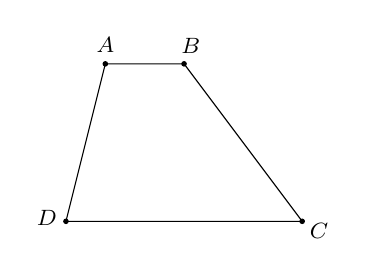
\begin{tikzpicture}[scale=1,font=\footnotesize,line join=round,line cap=round,>=stealth]
\foreach \x/\y/\t in {0.5/2/A,1.5/2/B,3/0/C,0/0/D}
\coordinate (\t) at (\x,\y);
\draw (A)--(B)--(C)--(D)--(A);
\foreach \t/\g in {A/90,B/70,C/-30,D/170}
\draw[fill=black] (\t)circle(0.8pt) +(\g:7pt)node{$\t$};
\end{tikzpicture}
}
}

\end{ex}

\begin{ex}%[VN-MT-9]%[0-TK-HK1-KN-8-2425, Nguyễn Quang Hiệp]%[0H5V3-9]
Phân tử sulfur dioxide ($\mathrm{SO}_2$) có cấu tạo hình chữ V, góc liên kết $OSO$ gần bằng $120^\circ$. Người ta biểu diễn sự phân cực giữa nguyên tử $S$ với mỗi nguyên tử $O$ bằng các vectơ $\overrightarrow{\mu}_1$ và $\overrightarrow{\mu}_2$, có cùng phương với liên kết cộng hóa trị, có chiều từ nguyên tử $S$ về mỗi nguyên tử $O$ và cùng có độ dài là $1{,}6$ đơn vị (Hình bên dưới).
\begin{center}
\begin{tikzpicture}[>=stealth,line join=round,line cap=round,font=\footnotesize,scale=1]
\tikzset{declare function={r1=.5;}}
\tikzset{pics/truc/.style n args={4}{
code={\tikzset{declare function={a=#1;b=#2;}}
\shade[left color=#3,right color=#4] (0,0)rectangle(a,b);}
}}
\path
(0,0)coordinate (A)--++(0:5)coordinate (B)
($(A)!.5!{30}:(B)$)coordinate (x) ($(B)!.5!{-30}:(A)$)coordinate (y)
(intersection of A--x and B--y) coordinate (C)
($(A)+(B)-(C)$)coordinate (D)
;

\path (0,-.2)pic[rotate=30]{truc={2.5}{.25}{red}{yellow}};
\path (5,0.1)pic[rotate=150]{truc={2.5}{.25}{yellow}{red}};
\shade[ball color=red] (A)coordinate (O)circle(r1)node[scale=2]{O};
\shade[ball color=red] (B)circle(r1)node[scale=2]{O};
\shade[ball color=yellow] (C)circle(r1)node[scale=2]{S};
\path
(A)--(C)node[above,pos=.5,sloped]{$\overrightarrow{\mu}_1$}
(B)--(C)node[above,pos=.5,sloped]{$\overrightarrow{\mu}_2$}
(C)--(D)node[right,pos=.5]{$\overrightarrow{\mu}$}
;
\draw[->,ultra thick,color=cyan](C)--(A);
\draw[->,ultra thick,color=cyan](C)--(B);
\draw[->,ultra thick,color=yellow](C)--(D);
\draw[cyan,dashed,ultra thick](A)--(D)--(B);
\end{tikzpicture}
\end{center}
Cho biết vectơ tổng $\overrightarrow{\mu}=\overrightarrow{\mu}_1+\overrightarrow{\mu}_2$ được dùng để biểu diễn sự phân cực của cả phân tử $\mathrm{SO}_2$. Tính độ dài của $\overrightarrow{\mu}$ (\textit{kết quả làm tròn đến một chữ số sau dấu phẩy}).
\shortans{1{,}6}
\loigiai{
\begin{center}
\begin{tikzpicture}[>=stealth,line join=round,line cap=round,font=\footnotesize,scale=1]
\tikzset{declare function={r1=.5;}}
\tikzset{pics/truc/.style n args={4}{
code={\tikzset{declare function={a=#1;b=#2;}}
\shade[left color=#3,right color=#4] (0,0)rectangle(a,b);}
}}
\path
(0,0)coordinate (A)--++(0:5)coordinate (B)
($(A)!.5!{30}:(B)$)coordinate (x) ($(B)!.5!{-30}:(A)$)coordinate (y)
(intersection of A--x and B--y) coordinate (C)
($(A)+(B)-(C)$)coordinate (D)
;

\path (0,-.2)pic[rotate=30]{truc={2.5}{.25}{red}{yellow}};
\path (5,0.1)pic[rotate=150]{truc={2.5}{.25}{yellow}{red}};
\shade[ball color=red] (A)coordinate (O)circle(r1)node[scale=2]{O};
\shade[ball color=red] (B)circle(r1)node[scale=2]{O};
\shade[ball color=yellow] (C)circle(r1)node[scale=2]{S};
\path
(A)--(C)node[above,pos=.5,sloped]{$\overrightarrow{\mu}_1$}
(B)--(C)node[above,pos=.5,sloped]{$\overrightarrow{\mu}_2$}
(C)--(D)node[right,pos=.5]{$\overrightarrow{\mu}$}
(A)--(D)node[above,pos=.5,sloped]{$\overrightarrow{\mu}_3$}
;
\draw[->,ultra thick,color=cyan](C)--(A);
\draw[->,ultra thick,color=cyan](C)--(B);
\draw[->,ultra thick,color=yellow](C)--(D);
\draw[cyan,dashed,ultra thick](A)--(D)--(B);
\end{tikzpicture}
\end{center}
Từ điểm cuối của vectơ $\overrightarrow{\mu}_1$ vẽ vectơ $\overrightarrow{\mu}_3=\overrightarrow{\mu}_2$, suy ra $\overrightarrow{\mu}=\overrightarrow{\mu}_1+\overrightarrow{\mu}_2=\overrightarrow{\mu}_1+\overrightarrow{\mu}_3$ nên $\left| \overrightarrow{\mu} \right|=\left| \overrightarrow{\mu}_1+\overrightarrow{\mu}_3 \right|$.\\
Ta có $\left( \overrightarrow{\mu}_1, \overrightarrow{\mu}_2 \right)=120^\circ $ nên $\left( \overrightarrow{\mu}_1, \overrightarrow{\mu}_3 \right)=60^\circ$.\\
Khi đó
\begin{align*}\left| \overrightarrow{\mu} \right|^2=\left| \overrightarrow{\mu}_1 \right|^2+\left| \overrightarrow{\mu}_3 \right|^2 - 2\left| \overrightarrow{\mu}_1 \right|\left| \overrightarrow{\mu}_3 \right| \cos \left( \overrightarrow{\mu}_1, \overrightarrow{\mu}_3 \right)
= 1{,}6^2+1{,}6^2 - 2 \cdot 1{,}6 \cdot 1{,}6 \cdot \cos 60^\circ=\frac{64}{25}\end{align*}
Suy ra $\left| \overrightarrow{\mu} \right|=\sqrt{\dfrac{64}{25}}=1{,}6$.\\
Vậy độ dài của $\overrightarrow{\mu}$ là $1{,}6$ đơn vị.
}
\end{ex}

\begin{ex}%[0D2V2-3]%[VN-MT6, Đào Trung Kiên]%[Sở Bắc Giang]
	Trong một cuộc thi pha chế, mỗi đội chơi được sử dụng tối đa $12$ gam hương liệu hòa tan, $9$ lít nước và $315$ gam đường để pha chế hai loại nước A và B. Để pha chế $1$ lít nước loại A cần $45$ gam đường, $1$ lít nước và $0,5$ gam hương liệu. Để pha chế $1$ lít nước loại B cần $15$ gam đường, $1$ lít nước và $2$ gam hương liệu. Mỗi lít nước loại A nhận được $60$ điểm thưởng, mỗi lít nước loại B nhận được $80$ điểm thưởng. Để đội chơi được số điểm thưởng là lớn nhất thì cần pha chế $a$ lít nước loại A và $b$ lít nước loại B. Tính tổng $a+b$.
	\shortans[]{$9$}
	\loigiai
	{Gọi $x$, $y$ lần lượt là số loại nước A và nước B mà đội chơi cần pha chế. \\
		Vì mỗi đội chơi được sử dụng tối đa $12$ gam hương liệu hòa tan nên ta có $0{,}5x+2y\leq 12$.\\
		Mỗi đội chơi được sử dụng tối đa $9$ lít nước nên ta có $x+y\leq 9$.\\
		Mỗi đội được sử dụng tối đa $315$ gam đường nên ta có bất phương trình $45x+15y\leq 315$.\\
		Từ đó ta có $\heva{&x\geq 0\\&y\geq 0\\ & 0{,}5x+2y\leq 12 \\ &x+y\leq 9 \\ & 45x+15y\leq 315} \Leftrightarrow \heva{&x\geq 0\\ &y\geq 0\\ &x+4y\leq 24\\ &x+y\leq 9\\ &3x+y\leq 21.}$ \hfill $(1)$ \\
		Số điểm thưởng là $f(x,y)=60x+80y$.\\
		\begin{center}
			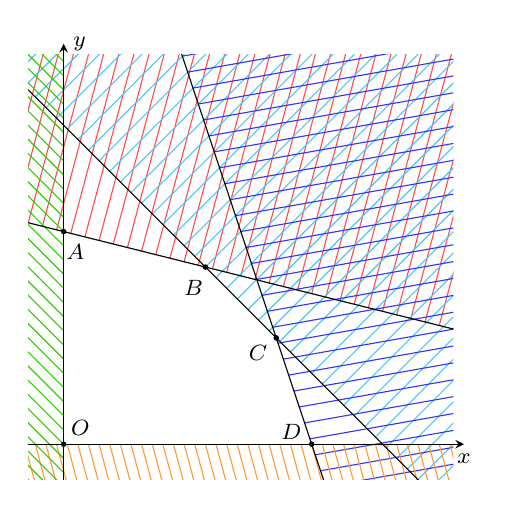
\begin{tikzpicture}[scale=1, font=\footnotesize, line join=round, line cap=round, >=stealth, x=0.45cm, y=0.45cm]
				\tikzset{declare function={f(\x)=6-0.25*(\x); g(\x)=9-\x; h(\x)=21-3*(\x);}}
				\def\xt{-1} \def\xp{11}
				\def\yd{-1} \def\yt{11}
				\begin{scope}
					\clip (\xt,\yd) rectangle (\xp,\yt);
					\foreach \i in {-3,-2.6,...,\xp} \draw[red!70!white] (\i,{f(\i)})--++(75:8);
					\foreach \j in {-2,-1.7,...,\xp} \draw[cyan!70!white] (\j,{g(\j)})--++(45:10);
					\foreach \k in {-1,-0.85,...,\xp} \draw[blue!80!white] (\k,{h(\k)})--++(10:8);
					\foreach \x in {-2,-1.7,...,\xp} \draw[orange!80!white] (\x,0)--++(-75:2);
					\foreach \y in {-2,-1.6,...,\yt} \draw[green!80!red] (0,\y)--++(135:2);
					\draw[domain=\xt:\xp] plot(\x,{f(\x)})
					plot(\x,{g(\x)})
					plot(\x,{h(\x)});
				\end{scope}	
				\draw[->] (\xt,0)--(\xp+0.3,0)node[below]{$x$};
				\draw[->] (0,\yd)--(0,\yt+0.3)node[right]{$y$};
				\foreach \p/\n/\g in {(0,0)/O/45, (0,6)/A/-60, (4,5)/B/-120, (6,3)/C/220, (7,0)/D/150} \fill \p node[shift={(\g:3mm)}]{$\n$} circle(1pt);
			\end{tikzpicture}
		\end{center}
		Miền nghiệm của hệ bất phương trình $(1)$ là ngũ giác $OABCD$ với $A(0;6)$; $O(0;0)$; $B(4;5)$, $C(6;3)$, $D(7;0)$. \\
		Vì giá trị lớn nhất của $f(x;y)=60x+80y$ đạt được tại đỉnh của miền nghiệm.\\
		Ta có $f(0;0)=0$, $f(0;6)=480$, $f(4;5)=640$, $f(6;3)=600$, $f(7;0)=420$.\\
		Suy ra $f(x,y)$ đạt giá trị lớn nhất tại $B(4; 5)$.\\
		Vậy để đạt số điểm thưởng lớn nhất đội chơi cần pha chế $9$ lít nước gồm $4$ lít nước loại A và $5$ lít nước loại B. 
	}
\end{ex}

\begin{ex}%[0D1V3-5]
Trường THPT Tài Đức tổ chức cho học sinh học thể dục dưới hình thức Câu lạc bộ, các học sinh đăng kí môn thể thao mà bản thân yêu thích. Lớp $10$A của trường có $24$ học sinh đăng kí môn bóng đá, $20$ học sinh đăng kí môn cầu lông, $7$ học sinh đăng kí cả hai môn bóng đá và cầu lông, $8$ học sinh đăng kí một môn khác. Hỏi sỉ số của lớp $10$A là bao nhiêu?
\shortans[4]{$45$}
\loigiai{
\begin{itemize}
\item Số học sinh chỉ đăng kí môn bóng đá là $24-7=17$ học sinh.
\item Số học sinh chỉ đăng kí môn cầu lông là $20-7=13$ học sinh.
\item Sĩ số của lớp 10A là $17+13+7+8=45$ học sinh.
\end{itemize}
}
\end{ex}
\Closesolutionfile{ans}
% \begin{indapan}
% 	{ans/0-HK1-CD-2-SoBacGiang-2324}
% \end{indapan}


\TL
\begin{ex}%[Đề thi HK1 THPT Nguyễn Chí Thanh 23-24]%[Phan Văn Thành - 10-11EX-HK12324]%[0H5H4-1]
Cho hình vuông $ABCD$ tâm $O$ có cạnh bằng $a$ và $M$ là trung điểm của $CD$, $E$ là trung điểm đoạn $AM$.
\begin{enumerate}
\item Biểu thị $\vec{AE}$ theo hai vectơ $\vec{AB}$ và $\vec{AD}$.
\item Tính tích vô hướng $\vec{AE} \cdot \vec{AC}$. Từ đó suy ra độ dài vectơ $\vec{AE}+\vec{AC}$.
\end{enumerate}
\loigiai{
\immini{\begin{enumerate}
\item Ta có $\vec{AE}=\dfrac{1}{2}\vec{AM}=\dfrac{1}{2}\left(\vec{AD}+\vec{DM}\right)=\dfrac{1}{2}\left(\vec{AD}+\dfrac{1}{2}\vec{DC}\right)=\dfrac{1}{2}\vec{AD}+\dfrac{1}{4}\vec{DC}=\dfrac{1}{4}\vec{AB}+\dfrac{1}{2}\vec{AD}$.
\item .
\end{enumerate}}{\begin{tikzpicture}[scale=1, font=\footnotesize, line join=round, line cap=round, >=stealth]

\path % khai báo tọa độ điểm
(0,0)coordinate(A)
(4,0)coordinate(B)
(4,4)coordinate(C)
(0,4)coordinate(D);
\coordinate (M) at ($(C)!0.5!(D)$);
\coordinate (O) at ($(B)!0.5!(D)$);
\draw (A)--(B)--(C)--(D)--(A) (A)--(M) (A)--(C) (B)--(D);% vẽ các đoạn thẳng liên tiếp
\foreach \p/\g in {A/-135,B/-45,C/45,D/135,M/90,O/-90} \draw[fill=white](\p)circle(1pt)node[shift={(\g:.3)}]{$\p$};
\end{tikzpicture}}

}
\end{ex}

\begin{ex}%[0H9C2-1]
Cho hình thang $ABCD$ vuông tại $A$ và $B$ có $AD \parallel BC$, $AB=AD=2$, $BC=6$. Gọi $E$ là giao điểm của $AC$ và $BD$, $F$ là điểm trên cạnh $BC$ sao cho $BF=\dfrac{1}{3}BC$, $G$ là trung điểm của $AB$. Khi đó $\widehat{GEF}$ có giá trị bằng bao nhiêu độ?
% \shortans{$90$}
\loigiai{
Do $\heva{&AD \parallel BC\\&AC \cap BD = E}$ nên $\dfrac{EB}{ED}=\dfrac{BC}{AD}=3$. Suy ra $EB=3ED$. Từ đó $\overrightarrow{BE}=\dfrac{3}{4}\overrightarrow{BD}$.\\
Xét hệ trục toạ độ $\left(O,\overrightarrow{i},\overrightarrow{j}\right)$ với $O \equiv B$, $\overrightarrow{i}=\dfrac{1}{2}\overrightarrow{BF}$ và $\overrightarrow{j}=\overrightarrow{BG}$. Ta có
\[B(0;0),\;G(0;1),\;F(2;0) \text{ và } D(2;2).\]
Do $\overrightarrow{BE}=\dfrac{3}{4}\overrightarrow{BD}$ nên $E\left(\dfrac{3}{2};\dfrac{3}{2}\right)$.\\
Như vậy $\heva{&\overrightarrow{EG}=\left(-\dfrac{3}{2};-\dfrac{1}{2}\right)\\&\overrightarrow{EF}=\left(\dfrac{1}{2};-\dfrac{3}{2}\right)}$, suy ra $\overrightarrow{EG}\cdot\overrightarrow{EF}=-\dfrac{3}{2}\cdot\dfrac{1}{2}+\left(-\dfrac{1}{2}\right)\cdot\left(-\dfrac{3}{2}\right)=0$ hay $EG \perp EF$.\\
Do đó $\widehat{GEF}=90^{\circ}$.
}

\end{ex}

\begin{ex}%[0D8C2-6]
Một đa giác đều có $32$ đỉnh. Có bao nhiêu cách chọn $3$ trong $32$ đỉnh để $3$ được chọn là $3$ đỉnh của một tam giác vuông nhưng không cân.
% \shortans[]{$113$}
\loigiai{
Đa giác đều có $32$ đỉnh sẽ có $16$ đường chéo đi qua tâm của đa giác (đường chéo chính).\\
Mà cứ $2$ đường chéo chính sẽ tạo thành $1$ hình chữ nhật. Cứ $1$ hình chữ nhật lại tạo thành $4$ tam giác vuông. Do đó, số tam giác vuông được tạo thành là $4\mathrm{C}_{16}^2=480$.\\
Mặt khác, trong số $\mathrm{C}_{16}^2$ hình chữ nhật lại có $8$ hình vuông. Suy ra, số tam giác vuông cân là $4\cdot 8=32$.\\
Vậy có $480-32=448$ cách chọn $3$ đỉnh để thành tam giác vuông mà không cân thoả yêu cầu bài toán.}
\end{ex}